% !TEX root = ../thesis.tex

\chapter{Web Processing Service}
\label{sec:wps}

The \acrocitep{WPS}{ogc:wps} is the quasi standard for web based processing of spatiotemporal data \citep{foerster2012live}. It is an open service standard specified by the \ac{OGC} and is embedded in the \ac{OWS} \citep{ogc:ows} environment. Even though the \ac{WPS} is mostly used in the geospatial domain, it's interface is not restricted to spatiotemporal data and also can be deployed in other professional contexts. Within the WPS, it is possible to publish and execute models, algorithms or generic calculations and computations in a standardized web service interface, so called processes. The \ac{WPS} describes a generic interface, that imposes no restrictions on the type of process, their inputs and outputs and so it can encapsulate any kind of algorithm or model. By this, an interoperability is offered, which leads to a number of significant advantages. It adds a layer that hides complexity and permits -- by it's consistency across implementations -- a high level of reusability, flexibility and scalability. Server and client software implementations become reusable and generic client implementations are possible. Scalable and complex computations, like grid \citep[e.g.][]{grid1,grid2,grid3} or cloud computing \citep[e.g.][]{cloud}, as well as super computer processing are hidden behind a simple to use service interface and become accessible.

The \ac{WPS} specifies mechanisms to discover algorithms and models by offering generic encoding formats for process descriptions and a uniform interface to explore and retrieve these. Besides that, it defines a universal process execution model, that includes request and response encodings, synchronous and asynchronous process executions, long running processes as well as a data encoding for input and output parameters. The interface offers the possibility to retrieve a process output either in a raw format, embedded in a response, or stored in the \ac{WPS} for later retrieval. This facilitates process chaining and enables the subsequent retrieval of process results. The specification describes three different bindings to access a \ac{WPS} using the \acrocitep{HTTP}{ietf:rfc2616}. It may be addressed using \ac{KVP} encoding with HTTP GET, XML encoding with HTTP POST, or clients may use SOAP \citep{w3c:soap1} to access the web service.

Functionalities are exposed by means of three distinct methods. As every \ac{OGC} web service the \ac{WPS} has a \emph{GetCapabilities} method, that can be used to request a detailed description of the service and its capabilities. It offers a service identification structure which contain information about the organization operating the \ac{WPS}. Also present is a service provider section that contains informational meta data about the service instance which can be used for service discovery. Besides that, detailed information about supported operations, bindings, languages as well as a list of available processes are incorporated.

The detailed description of a single process may be requested by using the \emph{DescribeProcess} operation. Its response contains informational meta data (like textual descriptions) and the process capabilities in regards to asynchronous execution and response/output storage. Comprehensive information about required and supported inputs, their cardinalities, supported formats and restrictions, and available outputs as well as their supported formats are also included.

Processes are executed using the \emph{Execute} operation. Besides the necessary input parameters and information about their encoding, the request describes selected outputs that should be generated by the process. Furthermore, it informs the \ac{WPS} whether the process should be executed synchronously or asynchronously and how the results of the process should be encoded.

\begin{figure}[!htb]
  \centering
  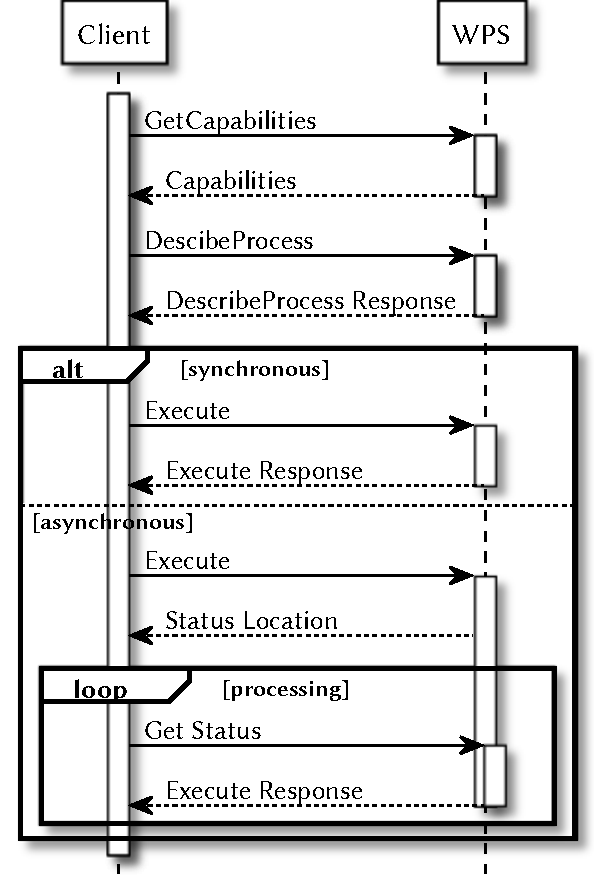
\includegraphics[width = 0.40140845070422537\linewidth]{figures/sequence-diagram-wps.pdf}
  \caption{\label{fig:sd:wps}Typical interaction patterns of the \acl{WPS}: process discovery using \emph{GetCapabilities} and \emph{DescribeProcess} and synchronous as well as asynchronous process execution using \emph{Execute}.}
\end{figure}

Typical interaction patterns of the \acl{WPS} are depicted in \cref{fig:sd:wps}. During process discovery, \emph{GetCapabilities} and \emph{DescribeProcess} are used to request a list of available processes and their descriptions. Process execution takes place either synchronously or asynchronously by issuing an \emph{Execute} request to a specific process. In the case of asynchronously process executions, the \ac{WPS} returns an URL to an \emph{ExecuteResponse} which is continuously updated and which the client can request periodically to get the current process status.

The \ac{WPS} describes three basic types of input and output parameters: \emph{literal}, \emph{complex} and \emph{bounding box} parameters. Complex data parameters are data structures that can be described by a mime type, an encoding and a schema. They can represent raster data, XML structures such as \ac{GML} \citep{ogc:gml} feature collections, \ac{CSV} or any other type of data. This data can be supplied embedded in XML or as a reference to an external HTTP resource. Referenced complex data structures may be requested by using HTTP GET or POST and can transport HTTP headers and any body payload (or reference to one). By this, chaining of \ac{WPS} processes can easily be implemented, either by referencing a previous generated output or even by encoding another \emph{Execute} call into the reference. Literal data can be represented by a single string value. The value is described by a data type and can be accompanied by a unit of measurement. Typical data types include single strings, URIs, boolean values, dates and integral or decimal numbers. Bounding box data represents a rectangular region of arbitrary dimension which is described by a \ac{CRS}.

As shown in this chapter, there are several benefits that can be expected by using the WPS. Especially in the context of domain specific models, the interoperability and reusability can be increased significantly. Until now, the \la can not be deployed in a web based processing chain and has to be executed in a manual procedure. Web based execution is currently realized by using a web form that allows remote execution of the \la. This way of proceeding presupposes the recourse to specialized software or scripts for automation and can be characterized as very disadvantageous, e.g. for the reuse of the developed model in other projects. The following section focuses on a WPS that allows the deployment of models developed in MATLAB -- like the \la -- as WPS processes with the purpose of profiting from the positive aspects of standardized web based processing solutions.